\documentclass[conference,10pt]{IEEEtran}
\IEEEoverridecommandlockouts
\usepackage[T1]{fontenc}
\usepackage{graphicx,booktabs,amsmath,amssymb,xcolor,url,xspace,textcomp}
\usepackage[hidelinks]{hyperref}
\hypersetup{pdftitle={G1Nav: Humanoid Locomotion RL with Hierarchical Target Navigation}, pdfauthor={Jeong Hwan Lee}}
\usepackage{array,tikz}
\usetikzlibrary{positioning,arrows.meta}
\def\UrlBreaks{\do\/\do\_\do\.\do\-}\def\UrlFont{\small\ttfamily}\newcommand{\code}[1]{\path{#1}}\newcommand{\cmd}[1]{\texttt{\detokenize{#1}}}
\definecolor{selF}{HTML}{E3F2FD}\definecolor{selS}{HTML}{1E88E5}
\definecolor{navF}{HTML}{FFFDE7}\definecolor{navS}{HTML}{F9A825}
\definecolor{polF}{HTML}{F3E5F5}\definecolor{polS}{HTML}{8E24AA}
\definecolor{simF}{HTML}{E8F5E9}\definecolor{simS}{HTML}{43A047}
\definecolor{logF}{HTML}{ECEFF1}\definecolor{logS}{HTML}{546E7A}

\begin{document}
\title{G1Nav: Humanoid Locomotion RL with\\Hierarchical Target Navigation\\[1mm]\Large A PPO Walking Policy for the Unitree G1 Driven by a Navigator in MuJoCo}
\author{\IEEEauthorblockN{Jeong Hwan Lee}
\IEEEauthorblockA{Technical report, status of 5 November 2026\\
Repository: \texttt{physical-ai-robot-learning/g1-target-walking}}}
\maketitle

\begin{abstract}
A simulated Unitree G1 humanoid receives an English instruction such as ``go to the red cube'' and walks to that object
in MuJoCo physics. The system is hierarchical: a slow stage selects the target once per episode, a hand-written
Navigator turns the target position and the robot's odometry into a velocity command every control step, and a
velocity-conditioned walking policy, trained from scratch with PPO in MuJoCo Playground's G1 Joystick environment (MJX),
outputs 29 lower-body PD joint targets at 50~Hz. Only the walking policy is learned. In the recorded demos the target is
chosen by keyword matching against the simulator's object labels and its position is simulator ground truth; a GR00T
N1.6 Eagle vision-language encoder runs on the start ego frame but its output is only logged. The question is therefore
the control half: can one walking policy, trained once, be driven by a simple Navigator to instructed targets in closed
loop? The policy was trained for 154.8~M environment steps (77~min). Re-evaluated in the raw environment, the first
checkpoint that walks is at 41.3~M steps, and the final policy moves at 0.52~m/s for a 0.6~m/s command with a minimum
torso height of 0.74~m. In all 3 demo scenes the robot reaches the instructed object (stop radius 0.55~m) without
falling; a CPU re-run reproduces the final distances. Getting there required domain randomisation, evaluating without the
training wrapper's auto-reset, and two deployment fixes to the observation (normalisation and the frame of the gravity
term). Three seeded scenes with one run each are a demonstration, not an evaluation: no success rate is reported.
\end{abstract}

% =====================================================================
\section{Introduction}\label{sec:intro}
Locomotion policies for humanoids are now routinely trained with reinforcement learning in massively parallel
simulation~\cite{rudin2022walk,zakka2025playground}. Such a policy usually tracks a velocity command; something else has to
decide where the robot should go. A common structure separates a slow decision about \emph{what} and \emph{where} from a
fast controller for balance and stepping. This report describes a small, complete instance of that structure for the
Unitree G1 in MuJoCo~\cite{todorov2012mujoco} and what it took to make the two halves work together.

\textbf{Main question.} \emph{Can one velocity-conditioned walking policy, trained once with RL, be driven by a simple
Navigator to reach instructed targets in closed loop, with physics only?} The target-selection half is deliberately
simple: a keyword rule over the simulator's object labels, with the object's ground-truth position. This report says
nothing about whether a vision-language model can do the grounding.

\textbf{Contributions.}
\begin{itemize}
\item a velocity-conditioned PPO walking policy for the G1, trained from scratch, with a re-evaluation of every saved
  checkpoint in the raw environment (Sec.~\ref{sec:loco}, \ref{sec:res-walk});
\item a Navigator and a deployment of the trained policy in a different scene, with an observation reproduced term by
  term from the training environment (Sec.~\ref{sec:nav}, \ref{sec:deploy});
\item closed-loop target reaching in three seeded scenes, re-measured on CPU from the committed checkpoint
  (Sec.~\ref{sec:res-loop});
\item the failures met on the way and their fixes (Sec.~\ref{sec:fail}).
\end{itemize}

\textbf{What is not shown.} No learned or visual grounding (the Eagle embedding is never used), no vision in the
control loop (this is not a vision-language-action model), no success rate, no new locomotion method (the
environment, reward and PPO hyperparameters are MuJoCo Playground's), and no hardware.

% =====================================================================
\section{Related work}\label{sec:related}
\textbf{Simulation and RL for legged locomotion.} MuJoCo~\cite{todorov2012mujoco} and its JAX implementation MJX make
thousands of parallel environments practical on one GPU; Brax~\cite{freeman2021brax} provides the PPO~\cite{schulman2017ppo}
implementation used here. Rudin et al.~\cite{rudin2022walk} showed that massively parallel PPO learns quadruped walking in
minutes. MuJoCo Playground~\cite{zakka2025playground} packages locomotion environments, including the G1 Joystick task
whose environment, reward and hyperparameters this work uses unchanged; its robot model comes from MuJoCo
Menagerie~\cite{menagerie2022}. Domain randomisation~\cite{tobin2017domain} is part of that recipe and turned out to be
necessary here (Sec.~\ref{sec:fail}).

\textbf{Vision-language backbones for robots.} GR00T N1~\cite{gr00t2025} is a vision-language-action model whose
vision-language part is an Eagle backbone. In this project the Eagle backbone of the GR00T N1.6 checkpoint is only run on
the start ego frame and its embedding statistics are logged; it was a placeholder for a learned grounding stage that was
not built.

% =====================================================================
\section{System}\label{sec:system}
\begin{figure}[t]
\centering
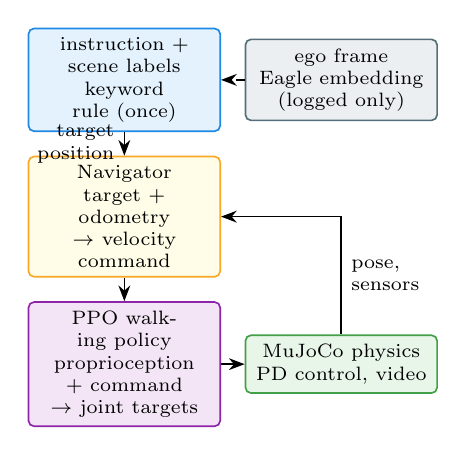
\begin{tikzpicture}[font=\scriptsize, node distance=3mm and 3mm,
  box/.style={draw, rounded corners=2pt, align=center, minimum height=7mm, text width=22mm, line width=0.6pt},
  arr/.style={-{Stealth[length=2mm]}, line width=0.6pt}]
\node[box, fill=selF, draw=selS] (sel) {instruction + scene labels\\keyword rule (once)};
\node[box, fill=logF, draw=logS, right=of sel] (eag) {ego frame\\Eagle embedding\\(logged only)};
\node[box, fill=navF, draw=navS, below=of sel] (nav) {Navigator\\target + odometry\\$\to$ velocity command};
\node[box, fill=polF, draw=polS, below=of nav] (pol) {PPO walking policy\\proprioception + command\\$\to$ joint targets};
\node[box, fill=simF, draw=simS, right=of pol] (sim) {MuJoCo physics\\PD control, video};
\draw[arr] (sel) -- node[left, align=right]{target\\position} (nav);
\draw[arr] (nav) -- (pol);
\draw[arr] (pol) -- (sim);
\draw[arr] (sim.north) |- node[right, pos=0.25, align=left]{pose,\\sensors} (nav.east);
\draw[arr, dashed] (eag.west) -- (sel.east);
\end{tikzpicture}
\caption{The hierarchy. Target selection runs once per episode; the Navigator, the policy and the physics run every
control step. The Eagle embedding (dashed) does not influence the target.}
\label{fig:arch}
\end{figure}

\textbf{Robot and simulator.} The robot is the Unitree G1 model of MuJoCo Playground (from MuJoCo Menagerie) with 29
actuated joints, controlled at 50~Hz with physics at 500~Hz (10 substeps per control step). Training runs in MJX; the
closed-loop demos run the same model in plain MuJoCo with the training environment's solver options
(Sec.~\ref{sec:deploy}).

\textbf{Scenes.} A seed determines a 6~m $\times$ 6~m arena with low walls, the robot's spawn at a wall facing inward,
and 3 coloured objects (ball, cube, cylinder or cone in one of six colours) at random range and bearing inside the
robot's frontal field of view, non-overlapping. The scene carries an ego camera on the torso and a fixed third-person
camera (Fig.~\ref{fig:ego}). The recorded demos use seeds 0, 1 and 2.

\textbf{Observation and action.} The policy observes the 103-D state of Playground's G1 Joystick environment: local
linear velocity (3), gyro (3), gravity in the pelvis-IMU frame (3), velocity command (3), joint angles relative to the
default pose (29), joint velocities (29), last action (29) and the cosine/sine of the gait phase (2). The critic
additionally sees a 216-D privileged state. The action is a 29-D vector applied as PD position targets,
$q^{\mathrm{target}} = q^{\mathrm{default}} + 0.5\,a$. The command $(v_x, v_y, \omega_z)$ is in the robot's heading frame.

\textbf{Networks} (read from the checkpoint). Policy MLP 103 $\to$ 512 $\to$ 256 $\to$ 128 $\to$ 58 (mean and scale of 29
actions); value MLP 216 $\to$ 512 $\to$ 256 $\to$ 128 $\to$ 1; a running observation normaliser is stored with the
parameters.

\begin{figure}[t]
\centering
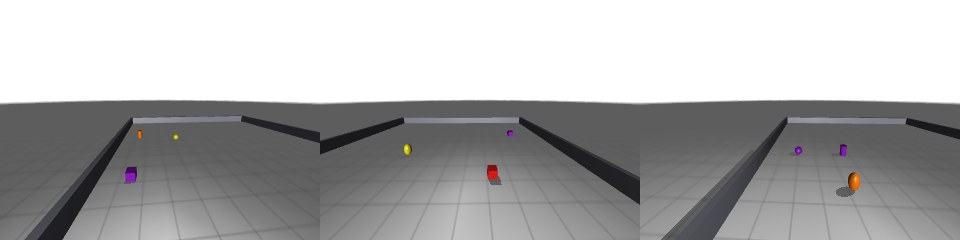
\includegraphics[width=\columnwidth]{figures/fig_ego_starts.jpg}
\caption{Start ego frames of the three demo scenes (seeds 0, 1, 2). Every object is in view at spawn.}
\label{fig:ego}
\end{figure}

% =====================================================================
\section{Method}\label{sec:method}
\subsection{Locomotion policy}\label{sec:loco}
The policy is trained with brax PPO on \texttt{G1JoystickFlatTerrain} with 8192 parallel environments, an asymmetric
critic and Playground's tuned hyperparameters. Following the official recipe, training uses Playground's domain
randomiser and a separate evaluation environment. The final run uses the default reward scales (termination $-100$,
linear-velocity tracking 1.0, stand-still $-1.0$). At every evaluation a checkpoint is saved and a short rollout with a
forward command is run in the raw environment. The run produced 16 checkpoints, 10{,}321{,}920 steps apart; the last is
at 154{,}828{,}800 steps.

\textbf{Raw-environment evaluation.} Every checkpoint is re-evaluated in the registry environment without the brax
training wrapper, so that a fall is a fall and not an automatic reset: command $v_x = 0.6$~m/s, 250 control steps
(5~s). Reported are the mean local forward velocity (the quantity the tracking reward uses), the net horizontal
displacement and the minimum torso height. A checkpoint ``walks'' if the forward velocity exceeds 0.3~m/s and the
torso stays above 0.4~m.

\subsection{Target selection}\label{sec:select}
The instructed target is the object label whose words occur most often in the lower-cased instruction, with ties broken
by label order; the target's world position is read from the generated scene. Each demo instruction names a unique
colour and shape, so this is a string match, not perception. The Eagle backbone embeds the start ego frame (286 tokens
$\times$ 2048-d) and the shape and norm of that embedding are logged.

\subsection{Navigator}\label{sec:nav}
The scene is static, so the target's world coordinate is fixed once and tracked with odometry (the robot's base pose).
Every control step the Navigator computes the bearing and distance to the target and issues a turn-then-go command: the
yaw rate is the bearing (rad) clipped to 0.5~rad/s; the forward speed is 0.45~m/s when the bearing is below 40.0$^\circ$ and
a quarter of that while turning, capped at 1.2 times the distance; no lateral command. Both channels are slew-rate
limited (0.04~m/s and 0.05~rad/s per step), because the policy topples on a step change in command. The robot stops
inside 0.55~m.

\subsection{Deployment in the navigation scene}\label{sec:deploy}
The navigation scene is Playground's G1 scene with the objects, walls and cameras injected. The policy only works there
if its inputs match training exactly. Three things had to be reproduced: the physics options (timestep, 3 solver
iterations, 5 line-search iterations, Euler integrator without Euler damping), the environment's hard-coded default
pose (not the keyframe's) for both the observation and the control, and the observation itself, read from the same
named sensors as in training, normalised with the stored running statistics, and with the gravity term computed in the
pelvis-IMU frame (Sec.~\ref{sec:fail}). Each episode holds a zero command for 2~s before navigation (and for 2~s after it when the target was reached),
ramps the command up over the first 25 control steps, and ends when the Navigator stops, when the torso drops below 0.4~m, or after
a 12~s budget.

% =====================================================================
\section{Experiments and results}\label{sec:results}
All numbers below are taken from committed files: the checkpoint pickles and training metrics in
\code{results/checkpoints/}, the CPU re-measurements in \code{results/} (made from the committed checkpoints; the
original GPU runs' logs are not in the repository), and the demo episode files in \code{media/}.

\subsection{Walking emergence}\label{sec:res-walk}
Table~\ref{tab:emergence} and Fig.~\ref{fig:emergence} show the evaluation reward of training and the raw-environment
re-evaluation of the checkpoints. Walking first appears at the 41.3~M checkpoint, where the evaluation reward also
crosses zero; from there every checkpoint walks. The highest forward velocity in the sweep is 0.58~m/s at 144.5~M steps;
the final policy moves at 0.52~m/s for the 0.6~m/s command (87~\%) and covers 2.59~m in 5~s. The training-time rollout
of the final checkpoint (4~s) gives 0.519~m/s, 2.07~m and a minimum torso height of 0.745~m. Throughput was about 2.3~M
steps/min between the first and the last evaluation and about 2.0~M steps/min over the whole run including compilation.

\begin{table}[t]
\centering
\caption{Walking emergence: evaluation reward of training and raw-environment re-evaluation (command 0.6~m/s, 5~s).}
\label{tab:emergence}
\setlength{\tabcolsep}{4pt}
\begin{tabular}{rrrrrl}
\toprule
step & reward & fwd vel & net dist & min $z$ & verdict\\
\midrule
0 & $-6.30$ & 0.36 & 0.45 & $-0.78$ & falls\\
10.3~M & $-2.83$ & 0.28 & 0.55 & $-0.78$ & falls\\
31.0~M & $-2.09$ & $-0.27$ & 0.76 & $-0.76$ & falls\\
\textbf{41.3~M} & \textbf{0.03} & \textbf{0.32} & \textbf{1.54} & \textbf{0.73} & \textbf{walks}\\
61.9~M & 3.99 & 0.50 & 2.51 & 0.73 & walks\\
144.5~M & 8.75 & 0.58 & 2.89 & 0.74 & walks\\
154.8~M & 9.29 & 0.52 & 2.59 & 0.74 & walks (final)\\
\bottomrule
\end{tabular}
\\[1mm]{\footnotesize Velocities in m/s, distances and heights in m. A negative min $z$ is a fallen robot.}
\end{table}

\begin{figure}[t]
\centering
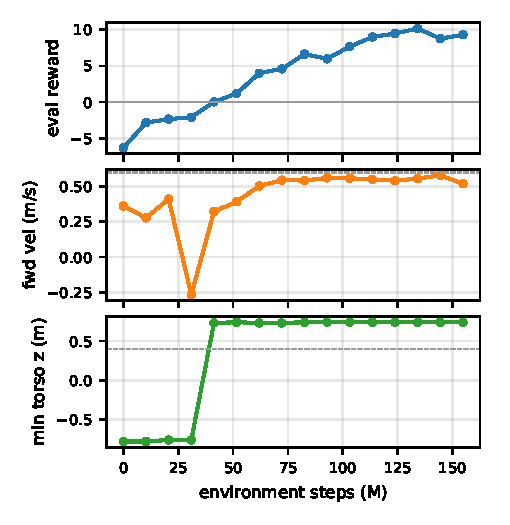
\includegraphics[width=\columnwidth]{figures/fig_emergence.pdf}
\caption{Per checkpoint: evaluation reward during training (top), and in the raw-environment re-evaluation the mean
forward velocity against the commanded value (middle, dashed) and the minimum torso height against the fall threshold
(bottom, dashed).}
\label{fig:emergence}
\end{figure}

\subsection{Closed-loop target reaching}\label{sec:res-loop}
Table~\ref{tab:loop} lists the three demo episodes. In each, the keyword rule selected the instructed object, and the
robot reached it without falling. ``Reached'' means that the Navigator's stop condition fired (planar distance at most
0.55~m); the final distance is measured after the standing post-roll. Seed 2 stops at 0.54~m against the 0.55~m radius.
Re-running the three episodes on CPU reproduces the final distances and torso heights to the printed precision; frame
counts match for seeds 0 and 2 and differ by one for seed 1 (386 vs 387). Fig.~\ref{fig:episode} shows the seed-0
episode.

\begin{table}[t]
\centering
\caption{Closed-loop demo episodes (one run per seed).}
\label{tab:loop}
\setlength{\tabcolsep}{3pt}
\begin{tabular}{rlccc}
\toprule
seed & instruction / chosen target & final dist & torso $z$ & frames\\
\midrule
0 & orange cylinder & 0.39 & 0.75 & 630\\
1 & red cube & 0.41 & 0.76 & 387\\
2 & purple cylinder & 0.54 & 0.75 & 668\\
\bottomrule
\end{tabular}
\\[1mm]{\footnotesize Instruction ``go to the $\langle$target$\rangle$''; all three reached, none fell. Distances and
heights in m; frames of the video.}
\end{table}

\begin{figure*}[t]
\centering
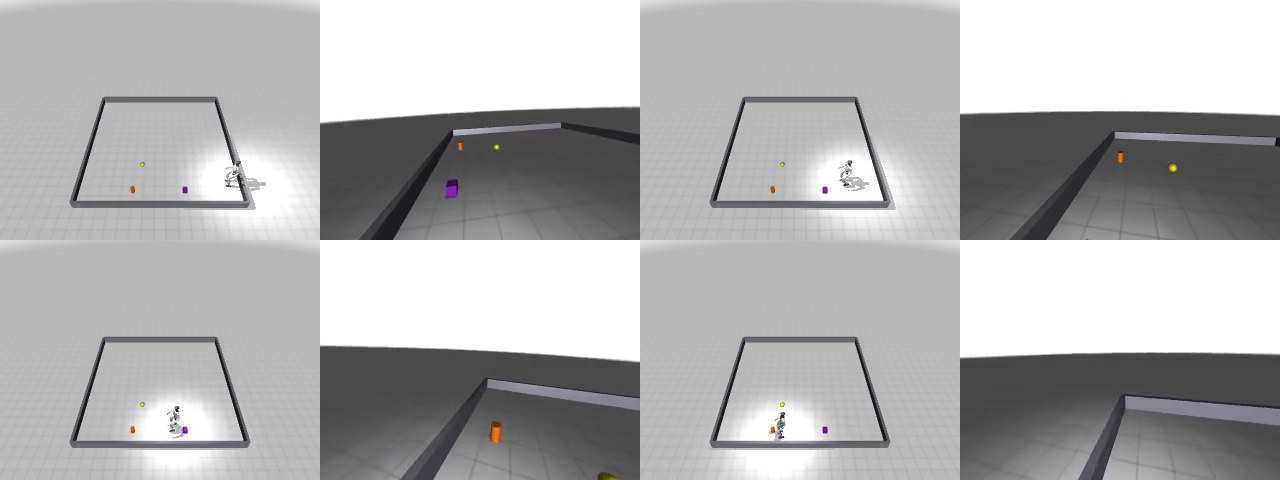
\includegraphics[width=0.68\textwidth]{figures/fig_episode.jpg}
\caption{``go to the orange cylinder'' (seed 0): third-person view and ego camera at the end of the standing pre-roll,
while turning, while approaching, and standing at the target (left to right, top to bottom).}
\label{fig:episode}
\end{figure*}

% =====================================================================
\section{Failure analysis}\label{sec:fail}
The engineering log below describes intermediate runs and code versions whose logs are not in the repository; it is
the author's record, not re-checkable results.

\textbf{Reward rises, the robot does not walk.} Without domain randomisation the evaluation reward increased but the
policy did not walk. Adding the domain randomiser and a separate evaluation environment made walking learnable.

\textbf{The ``marches in place'' illusion.} With a softened termination penalty ($-3$) the policy reached a high reward
($+19$) by marching in place: with falling almost free, stepping safely collects the air-time, phase, posture and
angular-tracking terms without forward motion. The in-training rollout hid the falls, because the training wrapper resets
the robot to the start pose on every fall, so a falling policy rendered as stable stepping. Restoring the default
termination penalty and evaluating every checkpoint in the raw environment fixed both.

\textbf{Observation mismatch.} Building the observation by hand from positions, velocities and the base quaternion made a
walking policy fall; reading the same named sensors as the training environment fixed it.

\textbf{The closed loop fell over.} The policy walked in the raw environment but toppled within about 1.6~s in the
navigation scene. Comparing the observation term by term with the training environment found two bugs. (a) Training
normalised observations, and the checkpoint stores the running statistics, but the deployment built the network without
the normaliser, so the policy saw raw observations; fixing this alone let the robot reach a target straight ahead.
(b) The gravity term of training is the world down vector expressed in the pelvis-IMU frame; the deployment used the
negated world-frame up vector, which coincides with it only while the robot walks straight. The robot fell on every
turn, exactly the symptom. With both fixes all three demo scenes are reached upright.

\textbf{Infrastructure.} The pinned JAX stack failed with a cuSolver internal error on an Ampere GPU and had no kernels
for Blackwell; training ran on an RTX 6000 Ada. Rendering a rollout video at every evaluation with too many evaluations
throttled training about 50$\times$; 50 evaluations over the run (one every $\sim$10~M steps) kept it fast.

% =====================================================================
\section{Limitations}\label{sec:limits}
Target selection is keyword matching and the target position is ground truth; instructions must name the object's colour
and shape, and nothing is learned or evaluated on the perception side. The results are three seeded scenes with one
run each, static objects and flat terrain: a demonstration, not an evaluation, and no success rate is reported. The
static-scene assumption fixes the target once. The walking policy follows the Playground recipe and reward; the
contribution is the coupling and the debugging. Everything is in simulation; no transfer to hardware was attempted.

% =====================================================================
\section{Reproducibility}\label{sec:repro}
\textbf{Layout.} All code is one Python package, \code{src/g1nav}: \code{envs} (seeded scenes, instruction templates),
\code{locomotion} (PPO training, raw-environment evaluation), \code{navigation} (keyword rule, Eagle logging, Navigator,
closed loop, demo re-run) and \code{apps} (dashboards). \code{results/} holds the checkpoints, the training metrics and
the CPU re-measurements; \code{media/} the demo videos, start ego frames and cognition files; \code{scripts/pod/} the
GPU-machine set-up and runners; \code{configs/envs/} the pinned requirement files; \code{archive/} unused code.

\textbf{Commands} (after \cmd{pip install -e .}):
{\scriptsize
\begin{verbatim}
# training (GPU), default reward scales
python -m g1nav.locomotion.train_walk \
  --termination -100 --track_lin 1.0 \
  --stand_still -1.0 --num_evals 50 \
  --out results/checkpoints/walk_t4
# raw-environment sweep of all checkpoints
python -m g1nav.locomotion.walk_eval \
  --sweep results/checkpoints 'walk_t4_step*.pkl'
# one episode, and the three demo episodes
python -m g1nav.navigation.pipeline --seed 0 \
  --instruction "go to the orange cylinder"
python -m g1nav.navigation.rerun_demo_episodes --cpu
\end{verbatim}}

\textbf{What needs what.} The claims checks and tests need only Python with numpy (\cmd{pip install -e ".[test]"}).
The closed-loop episodes and the checkpoint sweep run on a CPU with the pinned simulation stack (\texttt{jax 0.5.3},
\texttt{brax 0.14.2}, \texttt{mujoco 3.4.0}, \texttt{playground 0.1.0}); an opt-in test re-runs both and compares them
with the committed files. Full-scale training needs an NVIDIA GPU. The Eagle encoder needs torch, a CUDA GPU and the
backbone, which is not redistributed.

\textbf{Number checks.} Every number in this report is taken from a file in the repository and checked by
\code{analysis/verify_report.py}; every number in the README by \code{analysis/verify_claims.py}. Both run in CI.

% =====================================================================
\section{Conclusion}\label{sec:conclusion}
A velocity-conditioned PPO walking policy, trained once from scratch, can be driven by a hand-written Navigator to
instructed targets in closed loop in physics simulation: in all 3 demo scenes the G1 reached the instructed object
without falling. The hard parts were not the hierarchy but the details: domain randomisation for learning, an evaluation
that cannot hide falls, and an observation at deployment that matches training term by term. The open question this
report does not answer is the other half: replacing the keyword rule and ground-truth position with perception, and
measuring a success rate over many scenes.

\begin{thebibliography}{9}
\bibitem{todorov2012mujoco} E.~Todorov, T.~Erez, and Y.~Tassa, ``MuJoCo: A physics engine for model-based control,'' in
  \emph{Proc. IEEE/RSJ IROS}, 2012, pp.~5026--5033.
\bibitem{freeman2021brax} C.~D. Freeman, E.~Frey, A.~Raichuk, S.~Girgin, I.~Mordatch, and O.~Bachem, ``Brax -- A
  differentiable physics engine for large scale rigid body simulation,'' in \emph{NeurIPS Datasets and Benchmarks}, 2021.
\bibitem{schulman2017ppo} J.~Schulman, F.~Wolski, P.~Dhariwal, A.~Radford, and O.~Klimov, ``Proximal policy optimization
  algorithms,'' arXiv:1707.06347, 2017.
\bibitem{rudin2022walk} N.~Rudin, D.~Hoeller, P.~Reist, and M.~Hutter, ``Learning to walk in minutes using massively
  parallel deep reinforcement learning,'' in \emph{Proc. Conf. Robot Learning (CoRL)}, 2021.
\bibitem{zakka2025playground} K.~Zakka \emph{et al.}, ``MuJoCo Playground,'' arXiv:2502.08844, 2025.
\bibitem{menagerie2022} K.~Zakka, Y.~Tassa, and MuJoCo Menagerie contributors, ``MuJoCo Menagerie: A collection of
  high-quality simulation models for MuJoCo,'' \url{https://github.com/google-deepmind/mujoco_menagerie}, 2022.
\bibitem{tobin2017domain} J.~Tobin, R.~Fong, A.~Ray, J.~Schneider, W.~Zaremba, and P.~Abbeel, ``Domain randomization for
  transferring deep neural networks from simulation to the real world,'' in \emph{Proc. IEEE/RSJ IROS}, 2017.
\bibitem{gr00t2025} NVIDIA \emph{et al.}, ``GR00T N1: An open foundation model for generalist humanoid robots,''
  arXiv:2503.14734, 2025.
\end{thebibliography}
\end{document}
